\section{Datenhaltung im Modellkern}

Der Modellkern, dessen Hauptaufgabe die Verwaltung der Daten darstellt, bildet den wichtigsten Bestandteil des Komponentenmodells mit den im Folgenden kurz erl�uterten Anforderungen.

\begin{itemize}
\item \textbf{Speicherung}\\
Der Modellkern muss in der Lage sein, alle Daten zur Laufzeit des nutzenden Programms zu speichern. Zu den Daten geh�ren die Entit�ten des Komponentenmodells mit ihren Attributen. Die Struktur der Attribute beschr�nkt sich hierbei nicht auschlie�lich auf Standartdatentypen. Es m�ssen beliebige z.T. zur Entwurfszeit unbekannte Datenstrukturen speicherbar sein. Weiterhin m�ssen die Beziehungen zwischen den Entit�ten (z.B. Komponente \emph{A} enth�lt Komponente \emph{B}) festgehalten werden. 

\item \textbf{Konsistenzpr�fung}\\
Wie eingangs in der Architekturbescheibung erl�utert besteht die Aufgabe des Modellkerns nicht in der Implementierung der Konsistenzpr�fung des theoretischen Modells. Somit sollte im Idealfall prinzipiell erst einmal alles abspeicherbar sein. Da die Umsetzung dieser Anforderung viele ungenutzte und zu Lasten der Komplexit�t fallende M�glichkeiten bietet, ist die Nutzung von Wissen �ber das theoretische Modell bei der Konzeption der Datenhaltung sinnvoll einzubringen. Verst��e gegen die sich hierraus ergebenen Beschr�nkungen sind dann jedoch durch den Modellkern abzufangen und entsprechend zu behandeln. Soll beispielsweise entsprechend dem o.g. Beispiel die Komponente \emph{B} der Komponente \emph{A} hinzugef�gt werden, so ist vom Modell diese Beziegung zu speichern. Setzt die gew�hlte Speicherstruktur hierbei das vorhandensein von Komponente A vorraus, so ist das durch den Modellkern sicherzustellen. Dieser kann dann entweder die Speicherung ablehnen oder selbst�ndig eine Komponente A erzeugen.

\item \textbf{Zugriffsmethoden}\\
Die dritte Anforderung an den Modellkern stellen die Zugriffsmethoden dar. Da in die Datenhaltung, wie oben erl�uert, nicht das vollst�ndige Wissen �ber das theoretische Modell zu implementieren ist, k�nnen keine hierauf zugeschnittenen Zugriffsmethoden zur Verf�gung gestellt werden. Es ist also eine Schnittstelle zu schaffen, die flexiblen Zugriff auf alle gespeicherten Daten bereitstellt. Bestehen im Modell der Datenhaltung bereits Beziehungen zwischen den Daten, so bietet sich deren Nutzung beim Zugriff an.
Weiterhin wichtig ist sowohl bei den Zugriffsmethoden als auch bei der Speicherung die Geschwindigkeit. Dieser Teil des Modells bildet, wie bereits erl�utert, die Datenhaltung f�r die laufende Anwendung. Sorgt die Arbeit auf dem Modell f�r zu hohe Latenz, so leidet die Nutzbarkeit der Anwendung hierrunter stark.

\end{itemize}

Zur Umsetzung des Modellkerns kommen eine Reihe von Strategien in Frage, von denen drei im Folgenden gegeneinander abgegrenzt werden. Abschlie�end folgt in diesem Kapitel die ausf�hrliche Vorstellung der in dieser Version des Komponentemodells implementierten Variante.

Die erste Strategie bedient sich ausschlie�lich objektorientierter Konzepte. Hierbei werden die Entit�ten durch Klasseninstanzen und Beziehungen zwischen diesen durch Referenzen auf andere Instanzen modelliert. Vorteile dieser Variante ergeben sich aus guter Modellierbarkeit von Spezialisierung, problemloser Speicherung von Attributen unbekannten Typs und hoher Geschwindigkeit. Erfahrungen haben gezeigt, dass sich bei der Umsetzung dieses Konzeptes Probleme hinsichtlich Wartbarkeit und Erweiterbarkeit ergeben, die sich auf die starke Abh�ngigkeit der Klassen untereinander zur�ckf�hren lassen. Ebenfalls schwierig zu modellieren sind auf diese Art zirkul�re Abh�nigkeiten.

Der zweite Ansatz bedient sich einer relationalen oder einer objektrelationalen Datenbank. Die Entit�ten werden hierbei in entsprechenden Tabellen der Datenbank gespeichert. Die Beziehungen zwischen den Entit�ten lassen sich in der Datenbank entsprechend als Beziehungen zwischen den Tabellen modellieren. Details zum Entwurf solcher Datenbankschemata und deren Nutzung sei an dieser Stelle auf entsprechende Literatur (z.b. \cite{lit:db}) verwiesen. 

\begin{figure}[ht]
 \centering 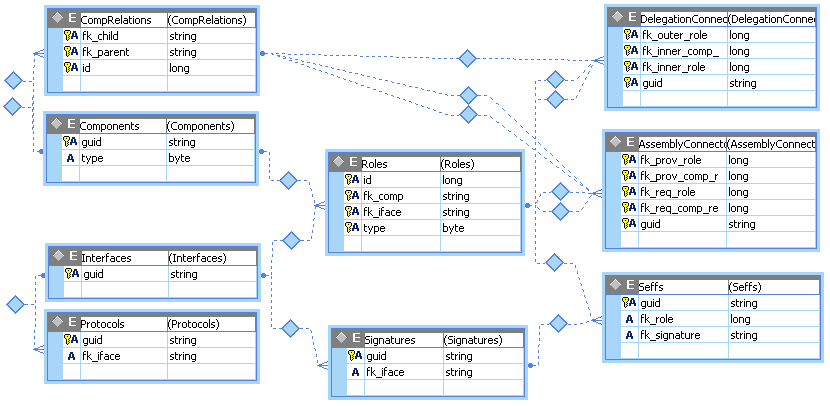
\includegraphics[scale=0.53]{dataset.png}
 \caption{.NET Dataset des Modellkerns}
 \label{fig:dataset}
\end{figure}